% !TEX root =  ../unref_general.tex
\section{Numerical Results}
\label{sec:Numerical}
This section illustrates the performance of our $hp$-adaptive strategy for a wide range of problems. We solve $2$D elliptic and non-elliptic problems based on Poisson, Helmholtz, and \revb{convection-diffusion} equations exhibiting multiple singularities. \rev{Additionally, we solve a $3$D non-elliptic problem based on a heterogeneous Helmholtz's equation.} For each example, we first display the results associated with the energy-norm adaptivity, followed by \rev{GOA} results. For all the experiments, we consider the Hilbert space $\H = \{u \in H^{1}(\Omega)  \, | \, u = 0 \text{ on } {\Gamma_{D}} \}$ , where $\Omega$ is the computational domain, and display the final adapted $h$- and $hp$-meshes and the convergence curves for $hp$-adaptivity and $h$-adaptivity with uniform $p=1$ and $p=2$. \revb{All the experiments start with a coarse mesh that is conforming to the materials and the source.}

We refer to $u$ as the solution in a fine grid, while $u_{\calT_{c}}$ is the solution associated with a coarser unrefined mesh. In energy-norm adaptivity, we define the relative error in percentage as:
\begin{equation}
  e_{\textrm{rel}}^{\textrm{energy}} \coloneqq  \frac{\norm{u - u_{\calT_{c}}}_{\H}}{\norm{u}_{\H}} \cdot 100.
  \label{eq:relerror}
\end{equation}
%\noindent The above quantity is difficult to compute in our data structures because we store a single grid at a time rather than maintaining several grids, which also facilitates the implementation. Thus, we estimate the following lower bound of the error $e_{\textrm{rel}}^{\textrm{energy}}$ as follows:
\noindent \rev{Rather than maintaining several grids, our easy-to-implement approach only stores a single grid at a time. Thus, we estimate the following lower bound of the error $e_{\textrm{rel}}^{\textrm{energy}}$ as follows:}
\begin{equation}
  \tilde{e}_{\textrm{rel}}^{\textrm{\, energy}} \coloneqq \frac{\abs{\norm{u}_{\H} - \norm{u_{\calT_{c}}}_{\H}}}{\norm{u}_{\H}} \cdot 100 \leq e_{\textrm{rel}}^{\textrm{energy}}.
  \label{eq:lowrelerror}
\end{equation}

We define the relative error in a QoI in percentage as follows:
\begin{equation}
  e_{\textrm{rel}}^{\textrm{QoI}} \coloneqq \frac{\abs{l(u) - l(u_{\calT_{c}})}}{\abs{l(u)}} \cdot 100.
  \label{eq:relerrorqoi}
\end{equation}
\noindent In some cases where the exact solution is available, we will replace the fine grid solution $u$ with the exact solution, and we will directly compute $e_{\textrm{rel}}^{\textrm{energy}}$ and $e_{\textrm{rel}}^{\textrm{QoI}}$.

\revb{For the GOA problems, we define our QoI as
  \begin{equation}
    l(\phi)=\frac{1}{\abs{\Omega_{l}}} \scalaire{\mathds{1}_{\Omega_{l}}}{ \phi}_{L^2(\Omega)}, \; \forall \phi \in \H,
    \label{eq:l_def}
  \end{equation}
}\noindent \reva{where  $\abs{\Omega_{l}}$ defines the area or volume of $\Omega_{l}$ and $\mathds{1}_{\Omega_{l}}$ is a function equal to one if $x \in \Omega_{l}$, and zero otherwise}.

\subsection{Singular Poisson example}
We consider the following elliptic problem based on the Poisson equation.
\begin{var_for}
  Find $u$ such that
  \begin{alignat}{2}
    - \Delta u & = \mathds{1}_{\Omega_{f}} &  & \text{ in } \Omega, \label{eq:poissongoal} \\
    u          & =0                        &  & \text{ on } {\partial \Omega},
  \end{alignat}
\end{var_for}
\noindent where $\Omega = (0,1) \times (\frac{1}{4},\frac{3}{4}) \cup (\frac{1}{4},\frac{3}{4}) \times (0,1) \subset \R^{2}$ \reva{and $\Omega_{f} = (\frac{1}{4},\frac{1}{2})^{2} \subset \Omega$}. \revb{Following the definition of \cref{eq:l_def} for the QoI, we select \reva{$\Omega_{l} = (\frac{1}{2},\frac{3}{4})^{2} \subset \Omega$}}. \Cref{fig:CrossGOAdomain} shows the domain $\Omega$ of this elliptic problem. For elliptic problems in energy-norm adaptivity, we refer the interested reader to \cite{darrigrand2020painless}. For goal-oriented adaptivity, \Cref{fig:CrossGOA_dir,fig:CrossGOA_adj} show the solutions of the direct and adjoint problems, respectively.

We define the operators $b(\cdot ,\cdot)$  and $a(\cdot ,\cdot)$ associated with the above problem as follows:
%\begin{align}
%  b(\cdot ,\cdot) & \coloneqq \sum_{K} \scalar{\grad \cdot}{\grad \cdot}_{L^{2}(K)}, & a(\cdot ,\cdot) & \coloneqq\sum_{K} \abs{\scalar{\grad \cdot}{\grad \cdot}_{L^{2}(K)}}.
%  \label{eq:forms_poisson}
%\end{align}
\rev{\begin{equation}
    b(\cdot ,\cdot)  \coloneqq   \scalar{\grad \cdot}{\grad \cdot}_{L^{2}(\Omega)},
    \label{eq:forms_poisson}
  \end{equation}
  and $a(\cdot ,\cdot) = b(\cdot ,\cdot)$.}
%Note that $\norm{\cdot}_e^2 =a(\cdot, \cdot)$ is our energy norm and $\abs{b(\phi,\psi)} \leq \abs{a( \phi,\psi)}, \, \forall \phi,\psi \in \H$.
%\noindent Then, we derive an upper bound of the error representation as follows:
%\begin{equation}
%  \label{eq:errQoiCross}
%  \abs{l(u_\calF)-l(u_{\calE_K})} \lesssim b (\Pi_{\calF}^{\calR_K} u_{\calF},\Pi_{\calF}^{\calR_K} v_{\calF}), \quad \forall K \in \calT.
%\end{equation}}


\noindent \Cref{fig:CrossGOA} shows the final $h$- and $hp$-adapted meshes and the evolution of $e_{\textrm{rel}}^{\textrm{QoI}}$. \revb{The first uniform mesh is composed of twelve root elements: given an initial $4 \times 4$ grid over a square domain, we have removed the four corner elements}. The grid adapts to the four localized reentrant corners of the domain. The $hp$-adaptive strategy performs $h$-refinements near these singularities and $p$-refinement as we move away from them, as physically expected. \revb{We also observe heavy refinements around the central point of the domain. That is the only point where the right-hand sides of the direct and adjoint problems are discontinuous; therefore, solutions of the direct and adjoint problems simultaneously exhibit low regularity (only $H^2$). Consequently, some refinements there are expected. Convergence rates of the proposed $hp$-adaptive strategy are quasi-optimal (see ~\Cref{fig:CrossGOA_error}).}

\begin{figure}
  \centering
  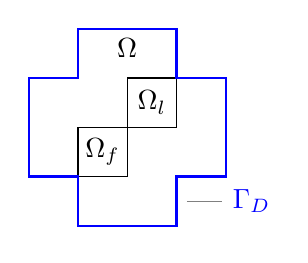
\begin{tikzpicture}[x=2.5cm,y=2.5cm]
    \node(n1) at (0.25,0){};
    \node(n2) at (0.75,0){};
    \node(n3) at (0.75,0.25){};

    \node(n4) at (0.25,0.25){};
    \node(n5) at (0.5,0.5){};
    \draw (n4) rectangle (n5) node[pos=0.5] {\reva{$\Omega_{f}$}};

    \node(n7) at (0.75,0.75){};
    \draw (n5) rectangle (n7) node[pos=0.5] {\reva{$\Omega_{l}$}};

    \draw[color=blue, thick,] (0.25,0) -- (0.75,0) -- (0.75,0.25) -- (1,0.25) -- (1,0.75) -- (0.75,0.75) -- (0.75,1) -- (0.25,1) -- (0.25,0.75) -- (0,0.75) -- (0,0.25) -- (0.25,0.25) -- (0.25,-0.005);
    \node(omega) at (0.5,0.90){$\Omega$};
    \draw[color=blue, thick] (n1.center) --  (n2.center) -- node[pos=0.5,pin={0: $\Gamma_{D}$}]{} (n3.center);
  \end{tikzpicture}
  \caption{Domain for our Poisson example. $\Gamma_{D}$ denotes the Dirichlet boundary, $\Omega$ is the domain, \reva{$\Omega_{l}$} denotes the support of the QoI $l(\phi)$, and \reva{$\Omega_{f}$} is the support of the source function.}
  \label{fig:CrossGOAdomain}
\end{figure}

\pagebreak

\begin{figure}
  \plothpGOA[unitsquare]{CrossGOA}{real}
  \caption{Direct and adjoint solutions of our singular Poisson example.}
\end{figure}

\pagebreak

\begin{figure}
  \plothp[hp,h]{CrossGOA}
  \caption{Final $h$- and $hp$-adapted meshes for our singular Poisson example and evolution of $e_{\textrm{rel}}^{\textrm{QoI}}$.}
  \label{fig:CrossGOA}
\end{figure}

\pagebreak

\subsection{\reva{Wave propagation problem}}
We consider the following non-elliptic problem based on Helmholtz's equation.
\begin{var_for}
  Find $u$ such that,
  \begin{alignat}{2}
    - \Delta u -k^{2}u   & = \mathds{1}_{\Omega_{f}} &  & \text{ in } \Omega,   \label{eq:helmholtzgoal} \\
    u                    & =0                        &  & \text{ on } {\Gamma_{D}},                      \\
    \grad u\cdot \vec{n} & =0                        &  & \text{ on } {\Gamma_{N}},
  \end{alignat}
\end{var_for}
\noindent where  $\Omega = (0,1)^{2} \setminus (\frac{1}{4},\frac{3}{4})^{2} \subset \R^{2}$, \reva{$\Omega_{f} = (0,\frac{1}{4})^{2} \subset \Omega$}, and $k = (8 \cdot 2 \pi, 2 \pi)$. The complex-valued $k$ indicates the \revbdos{medium} is lossy. $\Gamma_{D}$ and $\Gamma_{N}$ stand for the parts of the boundary $\partial \Omega$ where we impose homogeneous Dirichlet and Neumann boundary conditions, respectively. \revb{From \cref{eq:l_def}, we define}  \reva{$\Omega_{l} = (\frac{3}{4},1)^{2} \subset \Omega$}.  \Cref{fig:Helm2DGOAdomain} shows the domain of this non-elliptic problem.

\begin{figure}
  \centering
  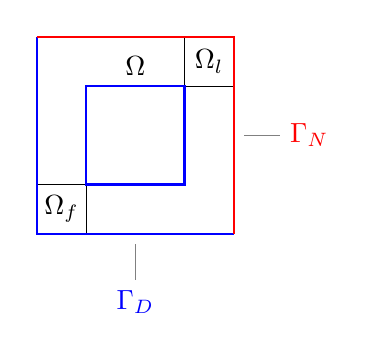
\begin{tikzpicture}[x=2.5cm,y=2.5cm]
    \node(n1) at (0,0){};
    \node(n2) at (1,0){};
    \node(n3) at (1,1){};
    \node(n4) at (0,1){};

    \node(n5) at (0.25,0.25){};
    \node(n6) at (0.75,0.25){};
    \node(n7) at (0.75,0.75){};
    \node(n8) at (0.25,0.75){};

    \draw (n1) rectangle (n5) node[pos=0.5] {\reva{$\Omega_{f}$}};
    \draw (n7) rectangle (n3) node[pos=0.5] {\reva{$\Omega_{l}$}};

    \draw[color=blue, thick] (n5) rectangle (n7);

    \draw[color=blue, thick] (n4.center) -- (n1.center) -- (n2.center) node[pos=0.5,pin={-90: $\Gamma_{D}$}]{};
    \draw[color=red, thick] (n4.center)--  (n3.center) -- node[pos=0.5,pin={0: $\Gamma_{N}$}]{} (n2.center);

    \node(omega) at (0.5,0.85){$\Omega$};

  \end{tikzpicture}
  \caption{Domain for our \reva{wave propagation problem}. $\Gamma_{D}$ denotes the Dirichlet boundary, $\Gamma_{N}$ stands for the Neumann boundary, $\Omega$ is the domain, \reva{$\Omega_{l}$} is the support of the QoI $l(\phi)$, and \reva{$\Omega_{f}$} is the support of the source function.
    \label{fig:Helm2DGOAdomain}}
\end{figure}

We define the operators $b(\cdot ,\cdot)$  and $a(\cdot ,\cdot)$ associated with the above problem as follows:
%\begin{align}
%  b(\cdot ,\cdot) & \coloneqq \sum_{K} \scalar{\grad \cdot}{\grad \cdot}_{L^{2}(K)} - k^2 \scalar{\cdot}{\cdot}_{L^{2}(K)},                           &
%  a(\cdot ,\cdot) & \coloneqq \sum_{K} \abs{\scalar{\grad \cdot}{\grad \cdot}_{L^{2}(K)}} + \abs{k^{2}} \abs{\scalar{\cdot}{\cdot}_{L^{2}(K)}}.
%  \label{eq:forms_singular}
%\end{align}
\rev{
  \begin{align}
    b(\cdot ,\cdot) & \coloneqq  \scalar{\grad \cdot}{\grad \cdot}_{L^{2}(\Omega)} - k^2 \scalar{\cdot}{\cdot}_{L^{2}(\Omega)},                    &
    a(\cdot ,\cdot) & \coloneqq \abs{\scalar{\grad \cdot}{\grad \cdot}_{L^{2}(\Omega)}} + \abs{k^{2}} \abs{\scalar{\cdot}{\cdot}_{L^{2}(\Omega)}}.
    \label{eq:forms_singular}
  \end{align}
}
Once more, $\norm{\cdot}_e^2 =a(\cdot, \cdot)$ defines our energy norm and $\abs{b(\phi, \psi)} \leq \abs{a(\phi, \psi)}, \, \forall \phi, \psi \in \H$.


\subsubsection{Energy-norm adaptivity}
%\tcr{Since the bilinear form $b$ of the problem does not define an inner product on $\H$, we introduce an alternative bilinear form $\tilde{b}$ as follows:
%\begin{equation}
%  \tilde{b}(\cdot, \cdot) = \sum_{K} \scalar{\grad \cdot}{\grad \cdot}_{L^{2}(K)} + \abs{k^{2}} \scalar{\cdot}{\cdot}_{L^{2}(K)}.
%\end{equation}
%\noindent Then, we define the element-wise indicator as:
%\begin{equation}
%  \eta_{K} \coloneqq \norm{\Pi_{\calF}^{\calR_K} u_\calF}^{2}_{e}, \quad \forall K \in \calT.
%\end{equation}}

For goal-oriented adaptivity, \Cref{fig:Helm2DGOA_dir,fig:Helm2DGOA_adj} show the solutions to the direct and adjoint problems, respectively. \Cref{fig:Helm2DGOANonmesh} shows the final $h$- and $hp$-adapted meshes and \Cref{fig:ErrorQoIenergy} shows the evolution of $\tilde{e}_{\textrm{rel}}^{\textrm{\, energy}}$ and $e_{\textrm{rel}}^{\textrm{QoI}}$. The initial uniform mesh is composed of twelve \revb{root} elements. We perform a double $h$-hierarchical refinement on the initial mesh to obtain a fine mesh to start the adaptivity.

For the $h$-adapted case, we observe heavy refinements around the source; however, almost no refinement occurs near the QoI. That happens due to the lossy nature of the problem. As a result, we observe a proper energy-norm convergence, as shown in  \Cref{fig:Helm2DGOANon_lower_com}, but a poor convergence behavior in the QoI, as demonstrated in  \Cref{fig:Helm2DGOANon_error_com}.

When executing the $hp$-adaptive strategy, we again observe heavier refinements around the source than in the vicinity of the QoI. However, because of the fast convergence of the $hp$-adaptivity, some non-trivial refinements still occur around the QoI. As a result, the relative error in the QoI $e_{\textrm{rel}}^{\textrm{QoI}}$ also converges up to the level of $10^{-3} \%$ for $20$k unknowns.

\pagebreak

\begin{figure}
  \plothpGOA[unitsquare]{Helm2DGOA}{abs}
  \caption{Absolute value of the direct and adjoint solutions of our \reva{wave propagation example} in a lossy \revbdos{medium}.}
\end{figure}

\pagebreak

\begin{figure}
  \plothpnon[hp,h]{Helm2DGOANon}
  \caption{Final $h$- and $hp$-adapted meshes for our \reva{wave propagation example} in a lossy \revbdos{medium}.}
  \label{fig:Helm2DGOANonmesh}
\end{figure}

\pagebreak

\begin{figure}
  \plothpcom[hp,h]{Helm2DGOANon}
  \caption{Energy-norm adaptivity. Evolution of $\tilde{e}_{\textrm{rel}}^{\textrm{\, energy}}$ and $e_{\textrm{rel}}^{\textrm{QoI}}$ in our \reva{wave propagation example} in a lossy \revbdos{medium}.}
  \label{fig:ErrorQoIenergy}
\end{figure}

\pagebreak

\subsubsection{Goal-oriented adaptivity}
%We introduce the following function $\hat{d}$:
%\begin{equation}
%  {\hat{d}} (\cdot ,\cdot) = \sum_{K} \abs{\scalar{\grad \cdot}{\grad \cdot}_{L^{2}(K)}} + \abs{k^{2}} \abs{\scalar{\cdot}{\cdot}_{L^{2}(K)}}.
%  \label{eq:hatd}
%\end{equation}
%\noindent Then, we derive an upper bound of the error representation as follows:
%\begin{equation}
%  \label{eq:errQoiHelmholtz}
%  \abs{l(u_\calF)-l(u_{\calE_K})} \lesssim \hat{d} (\Pi_{\calF}^{\calR_K} u_{\calF},\Pi_{\calF}^{\calR_K} v_{\calF}), \quad \forall K \in \calT.
%\end{equation}

\Cref{fig:Helm2DGOA} shows the final $h$- and $hp$-adapted meshes and the evolution of $e_{\textrm{rel}}^{\textrm{QoI}}$. The initial mesh is uniform and composed of twelve \revb{root} elements. As in the energy-norm adaptivity, we perform a double $h$-hierarchical refinement on the initial mesh to obtain a fine mesh to start the adaptivity. We observe heavy $h$-refinements around four localized singularities at the interior corners of the domain. In addition, we recover \revb{exponential} convergence rates for the $h$- and for the $hp$-adaptive versions. As a result, we construct a $hp$-adapted mesh with $20$k unknowns that delivers a relative error in the QoI of $10^{-6} \%$ (three orders of magnitude better than in \Cref{fig:Helm2DGOANon_error_com}).

\pagebreak

\begin{figure}
  \plothp[hp,h]{Helm2DGOA}
  \caption{Final $h$- and $hp$-adapted meshes for our singular goal-oriented wave propagation example in a lossy \revbdos{medium} and the evolution of $e_{\textrm{rel}}^{\textrm{QoI}}$.}
  \label{fig:Helm2DGOA}
\end{figure}

\pagebreak

\noindent To better illustrate this idea, \Cref{fig:comparison} compares the evolution of $e_{\textrm{rel}}^{\textrm{QoI}}$ and $\tilde{e}_{\textrm{rel}}^{\textrm{\, energy}}$ when executing the energy-norm and the goal-oriented $hp$-adaptive strategies in our \reva{wave propagation example} in a lossy medium. \Cref{subfig:compagoal} shows a relative error in the QoI three orders of magnitude better when performing goal-oriented adaptivity than considering energy-norm adaptivity. \Cref{subfig:compaenergy} shows that the $\tilde{e}_{\textrm{rel}}^{\textrm{\, energy}}$ rapidly converges when employing energy-norm adaptivity, while with the $hp$-adaptive GOA strategy, the rapid initial convergence stagnates at the level of $10^{-6} \%$. As expected, this situation is also noticeable in terms of $h$-adaptivity (see \Cref{fig:ErrorQoIenergy,fig:Helm2DGOA_error}).

\begin{figure*}[t!]
  \centering
  \begin{subfigure}[t]{0.5\textwidth}
    \centering
    \begin{tikzpicture}
      \begin{axis}[name=mainerrorplot,
          xlabel={Number of DoFs, $N$},
          %xlabel={dof per wavelength},
          %x dir=reverse,
          ylabel=Relative error in \% (log scale),
          ymode=log,
          xmode=log,
          %ymin=10e-12,
          %ymax=10e4,
          %xmax=5e4,
          %xmin=5e0,
          %yticklabel pos=right,
          ylabel near ticks,
          xlabel near ticks,
          enlargelimits=true,
          legend style={draw=black,fill=white,legend cell align=left, at={(0.5,1.01)}, anchor=south}, %Celda sobre plot (d)
          legend columns=-1
          %legend columns=4,
          %transpose legend,
          %legend columns=10,
          %reverse legend,
        ]

        %select coords between index={0}{20}

        \addplot+ [] table[x =nr_dof,y=Error ]{Figures/Helm2DGOA/hp/order_1/outputs.txt} ;
        \addlegendentry{GOA} \label{fig:item:qoigoa}

        \addplot+ [] table[x =nr_dof,y=Error ]{Figures/Helm2DGOANon/hp/order_1/outputs.txt} ;
        \addlegendentry{energy-norm}

      \end{axis}
    \end{tikzpicture}
    \caption{Evolution of goal-oriented adaptivity.}
    \label{subfig:compagoal}
  \end{subfigure}%
  ~
  \begin{subfigure}[t]{0.5\textwidth}
    \centering
    \begin{tikzpicture}
      \begin{axis}[name=mainerrorplot,
          xlabel={Number of DoFs, $N$},
          %xlabel={dof per wavelength},
          %x dir=reverse,
          %ylabel=Relative error in \% (log scale),
          ymode=log,
          xmode=log,
          %ymin=10e-12,
          %ymax=10e4,
          %xmax=5e4,
          %xmin=5e0,
          yticklabel pos=right,
          ylabel near ticks,
          xlabel near ticks,
          enlargelimits=true,
          legend style={draw=black,fill=white,legend cell align=left, at={(0.5,1.01)}, anchor=south}, %Celda sobre plot (d)
          legend columns=-1
          %legend columns=4,
          %transpose legend,
          %legend columns=10,
          %reverse legend,
        ]

        %\addplot+ [select coords between index={0}{27}]

        \addplot+ [] table[x =nr_dof,y=Lower ]{Figures/Helm2DGOA/hp/order_1/outputs.txt} ;
        \addlegendentry{GOA}

        \addplot+ [] table[x =nr_dof,y=Lower ]{Figures/Helm2DGOANon/hp/order_1/outputs.txt} ;
        \addlegendentry{energy-norm}

      \end{axis}
    \end{tikzpicture}
    \caption{Evolution of energy-norm adaptivity.}
    \label{subfig:compaenergy}
  \end{subfigure}
  \caption{Convergence history of $e_{\textrm{rel}}^{\textrm{QoI}}$ and $\tilde{e}_{\textrm{rel}}^{\textrm{\, energy}}$ for the energy-norm and GOA $hp$-adaptive strategies.}
  \label{fig:comparison}
\end{figure*}

\pagebreak

\subsection{Convection-dominated \reva{diffusion}: example 1}
We consider the following non-elliptic problem based on the \revb{convection-dominated diffusion} equation.
\begin{var_for}
  Find $u$ such that,
  \begin{alignat}{2}
    -\eps \Delta u + \sigma \cdot \grad u & = f &  & \text{ in } \Omega, \label{eq:convection} \\
    u                                     & =0  &  & \text{ on } {\partial \Omega}. \nonumber
  \end{alignat}
\end{var_for}

The selection of a suitable norm to measure the error in problems based on \cref{eq:convection} is an open research subject. For instance, authors of  \cite{franz2008superconvergence,franz2010local} use the standard energy norm, in \cite{franz2014error} a balanced norm, and in \cite{stynes2003sdfem,verfurth2005robust} different norms from the previous ones.  In here, we define the operators $b(\cdot ,\cdot)$ and  $a(\cdot ,\cdot)$ associated with the above problem as follows:
%\begin{align}
%  b(\cdot ,\cdot) & \coloneqq \sum_{K} \eps\scalar{\grad \cdot}{\grad \cdot}_{L^{2}(K)} +  \scalar{\sigma\grad\cdot}{\cdot}_{L^{2}(K)}, & a(\cdot ,\cdot) & \coloneqq \sum_{K} \abs{\eps+\frac{\abs{h_{K}}_{2}}{\abs{p_{K}}_{2}}\frac{\sigma \otimes\sigma}{\abs{\sigma}_{2}} \cdot \scalar{\grad \cdot}{\grad \cdot}_{L^{2}(K)}},
%  \label{eq:form_convection}
%\end{align}
\rev{
  \begin{align}
    b(\cdot ,\cdot) & \coloneqq \eps\scalar{\grad \cdot}{\grad \cdot}_{L^{2}(\Omega)} +  \scalar{\sigma\grad\cdot}{\cdot}_{L^{2}(\Omega)}, & a(\cdot ,\cdot) & \coloneqq (\eps + C) \scalar{\grad \cdot}{\grad \cdot}_{L^{2}(\Omega)},
    \label{eq:form_convection}
  \end{align}
}
\noindent where $\norm{\cdot}_e^2 =a(\cdot, \cdot)$ is our energy norm \rev{and $C \in \R^+$. We select this definition of $a(\cdot ,\cdot)$ by bounding from above the convective term of $b(\cdot ,\cdot)$ using a mesh-independent constant $C$ for the Poincaré inequality that also includes the effect of $\sigma$} \footnote{\rev{It is essential to consider a mesh-independent norm $a(\cdot, \cdot)^{1/2}$ since we approximate some errors by computing the difference of the norm of two approximated solutions evaluated on {\em different} grids.}} \footnote{\rev{The actual value of the constant C is unneeded in practice since we compute relative error indicators; in our case, we select $(C+\epsilon)=1$.}}. }







%b) Decir que vamos a obtener un upper bound de 42 usando una desigualdad de Poincaré que es mesh-independent, y ya por el mismo precio, independiente de tu coeficiente de difusión sigma. Como calculamos errores relativos, la constante al final no entra en ningún sitio y nos da igual la que pongamos. Es decir, que nuestra Ec. 42 acaba siendo tan sencilla como suma_K |(grad u, grad u)_K|
%
%Y si haces b), funciona. Y no solo eso, sino que luego calculas el error usando la Ec. 42 y más o menos va bastante bien. Al menos para el ejemplo que teníamos de 10^-4, con el sigma que teniamos y la fuente que la hemos hecho más cercana a la pared poniendo un cuadrado en muchos de los términos (Julen lo acaba de hacer).



\subsubsection{Energy-norm adaptivity}

For this example, we consider $\eps= 10^{-3}$ as the diffusive coefficient, $\sigma=(3,1)^{\text{T}}$, and $\Omega=(0,1)^{2}$. The load function $f$ is a linear continuos form on $\H$ and it is selected so that the solution $u$ is of the form:
\begin{equation}
  u(x,y) = \displaystyle{e^{\frac{\eps}{x (x - 1)} } \cosh \Big(500 \big(\frac{1}{2} + \sigma^{-1} (x, -y)\big) \Big)^{-2}.}
\end{equation}
%\tcr{We use the following bilinear form $\tilde{b}$:
%\begin{equation}
%  \label{eq:vcinternal}
%  \tilde{b}(\cdot, \cdot) = \sum_{K} \left(\eps+\frac{\abs{h_{K}}_{2}}{\abs{p_{K}}_{2}}\frac{\sigma \otimes\sigma}{\abs{\sigma}_{2}} \right) \scalar{\grad \cdot}{\grad \cdot}_{L^{2}(K)},
%\end{equation}
%\noindent where $h_{K}$ is the length of the element, and $p_{K}$ is the polynomial order. Then, we define the element-wise indicator as:
%\begin{equation}
%  \eta_{K} \coloneqq \norm{\Pi_{\calF}^{\calR_K} u_\calF}^{2}_{e}, \quad \forall K \in \calT.
%\end{equation}}

\Cref{fig:soltointBL} shows the solution of this convection-dominated \reva{diffusion} example. The initial uniform mesh is composed of thirty-six \revb{root} elements. \Cref{fig:intBL} shows the final energy-norm $h$- and $hp$-adapted meshes and the evolution of $e_{\textrm{rel}}$. As expected, we observe heavy $h$-refinements around the line that characterizes the solution. In the $hp$-adapted case, we also observe an increase in the polynomial order in some of the elements near this characteristic line. We also observe \revb{exponential} convergence rates (see \Cref{fig:intBL_error}).

\pagebreak

\begin{figure}
  \plothpDsol[unitsquare]{intBL}
  \caption{Solution of the convection-dominated \reva{diffusion} example 1.}
  \label{fig:soltointBL}
\end{figure}

\pagebreak

\begin{figure}
  \plothp[hp,h]{intBL}
  \caption{Final $h$- and $hp$-adapted meshes for our convection-dominated \reva{diffusion} example and the evolution of $e_{\textrm{rel}}^{\textrm{energy}}$.}
  \label{fig:intBL}
\end{figure}

\pagebreak

\subsection{Convection-dominated \reva{diffusion}: example 2}

\rev{We now consider a more challenging setting with advection skew to the mesh. We solve a similar problem to the one depicted in Figure 9.3 of~\cite{cottrell2009isogeometric} (see \Cref{fig:ConDiff2DGOA_setting}). Our convection-dominated diffusion problem is governed by \cref{eq:convection} on the domain $\Omega=(0,1)^{2}$, with $\eps= 10^{-4}$, $\sigma=(\cos \theta,\sin \theta)^{\textrm{T}}$, $\theta = \arctan(2)$, and zero Dirichlet boundary conditions, as depicted in \Cref{fig:ConvDiff2DGOANondomain}.}

\begin{figure}
  \centering
  \begin{subfigure}[b]{0.4\textwidth}
    \centering
    \begin{tikzpicture}[x=4.5cm,y=4.5cm]
      \node(n1) at (0,0){};
      \node(n2) at (1,0){};
      \node(n3) at (1,1){};
      \node(n4) at (0,1){};

      \node(n6) at (0.25,0.25){};
      \node(n7) at (0.25,0.5){};
      \node(n8) at (0,0.5){};
      \node(n9) at (0.75,0.75){};
      \node(n10) at (1,0.25){};
      %		\node(n11) at (1.05,0.5){};
      %
      \draw (n9) rectangle (n3) node[pos=0.5] {$\Omega_{l}$};

      \draw[color=blue, thick] (n2.center) -- (n3.center) -- (n4.center) -- (n8.center) node[pos=0.5,pin={180: $u=0$}]{};
      \draw[color=blue, thick] (n8.center) -- (n1.center) -- (n2.center) ;
      %		\draw[color=red,waved, thick] (n8.center) -- (n1.center) -- (n2.center) ;

      \draw[-] (n8.center) -- (n7.center) -- (n6.center) -- (n10.center);

      \node(omega) at (0.5,0.5){$\Omega$};
      \node(omega) at (0.5,0.125){$\Omega_{f}$};

    \end{tikzpicture}
    \caption{Problem setting.}
    \label{fig:ConvDiff2DGOANondomain}
  \end{subfigure}
  \hspace{0.05cm}
  \begin{subfigure}[b]{0.55\textwidth}
    \centering
    \plothpSource[unitsquare]{ConvDiff2DGOANon}
    \caption{Illustration of $f$ in  \cref{eq:convection}.}
    \label{fig:ConDiff2DGOANon_source}
  \end{subfigure}
  \caption{Problem description for our second convection-dominated diffusion with advection skew to the mesh.}
  \label{fig:ConDiff2DGOA_setting}
\end{figure}
\rev{We define our source term $f$ (with support in $\Omega_f$ and illustrated in \Cref{fig:ConDiff2DGOANon_source}) as:
  \begin{equation}
    f(x,y) = \begin{cases}
      (1-4x)^2,                                  & \text{if } x \in [0,0.25], y \in [0.25,0.5], \\
      (1-4y)^2,                                  & \text{if } x \in [0.25,1], y \in [0,0.25],   \\
      (1-4x) (1-4y) + (1-4y)^2 4x + (1-4x)^2 4y, & \text{if } x \in [0,0.25], y \in [0,0.25],   \\
      0,                                         & \text{otherwise.}
    \end{cases}
  \end{equation}
  Both the problem of Figure 9.3 of~\cite{cottrell2009isogeometric} and our problem share a strong boundary layer along the top and right boundaries of the domain. In addition, our problem incorporates (a) a source discontinuity on the edge $0 \leq x \leq 0.25, y =0.5$ that is visible in \Cref{fig:ConDiff2DGOANon_source}, and (b) a strong boundary layer for the adjoint problem along the bottom border of the domain. Thus, our example exhibits strong gradients of different (unknown) intensities in various areas of the domain, which makes it ideal for assessing the performance of our proposed $hp$-adaptive algorithm. The initial uniform mesh consists of $4 \times 4$ root elements for both adaptive strategies.}

%\begin{figure}
% \plothpSource[unitsquare]{ConvDiff2DGOANon}
%  \caption{Definition of $f$ in  \cref{eq:convection}. Redish colors represent higher values.}
%  \label{fig:ConDiff2DGOANon_source}
%\end{figure}


\subsubsection{Energy-norm adaptivity}


\rev{\Cref{fig:DirectsoltoConDiff2DGOANon} displays the final solution of the convection-dominated diffusion example 2 for the energy-norm adaptivity. \Cref{fig:ConvDiff2DGOANonmesh} shows the final energy-norm $h$- and $hp$-adapted meshes and the evolution of the relative error when using energy-norm adaptivity. As expected, $h$ and $hp$ meshes exhibit strong $h$-refinements towards the two boundary layers on the top and right sides of the domain. In addition, the $hp$-adaptivity is also able to capture both the advection propagation direction and the source discontinuity.}

\begin{figure}
  \plothpDsol[unitsquare]{ConvDiff2DGOANon}
  \caption{\reva{Numerical solution of the convection-dominated diffusion example 2 for energy-norm adaptivity.}}
  \label{fig:DirectsoltoConDiff2DGOANon}
\end{figure}


\begin{figure}
  \plothpnon[hp,h]{ConvDiff2DGOANon}
  \caption{Final $h$- and $hp$-adapted meshes for our convection-dominated diffusion example 2 and the evolution of $\tilde{e}_{\textrm{rel}}^{\textrm{\, energy}}$.}
  \label{fig:ConvDiff2DGOANonmesh}
\end{figure}

\pagebreak

\rev{\Cref{fig:mesheseachiteration1,fig:mesheseachiteration2} illustrate the evolution of the energy-based adaptive process by displaying at different iterations several solutions to the problem (left panels) and their corresponding $hp$-adaptive meshes (right panels). These meshes only display the polynomial orders in the $x$-direction, but analogous results are obtained for the $y$-direction. We accentuate the capability of the proposed algorithm to eliminate degrees of freedom previously introduced during the pre-asymptotic regime due to spurious oscillations. For instance, at iteration 7 (\Cref{fig:ConvDiff2DGOANon_007_iter_mesh}), high polynomial orders $p$ are set on the center-right part of the domain to capture the numerical artifacts exhibited by the solution (\Cref{fig:ConvDiff2DGOANon_007_iter_sol}). Once we better solve the problem, the numerical pollution starts to vanish (\Cref{fig:ConvDiff2DGOANon_010_iter_sol}), and consequently, some previously introduced high-order elements are $p$-unrefined (see \Cref{fig:ConvDiff2DGOANon_010_iter_mesh}) on the elements near the center of the domain and close to the right boundary layer.}

\rev{We also highlight the gradual behavior of the adaptive process: at the beginning, the refinements are mostly introduced to capture the boundary layers (\Cref{fig:ConvDiff2DGOANon_010_iter_mesh}). Once the boundary layers are properly resolved (\Cref{fig:ConvDiff2DGOANon_017_iter_mesh}), the algorithm refines to catch better the direction of propagation of the convection part of the problem. The adaptive process is almost finished at this point, and the error is of the order of $10^{-4}\%$. The final refinements are devoted to improving the solution nearby the source discontinuity, and accordingly, we begin to observe more refinements towards this region (see \Cref{fig:ConvDiff2DGOANon_021_iter_mesh}). The final meshes (iteration 27) correspond to \Cref{fig:ConvDiff2DGOANon_X_final,fig:ConvDiff2DGOANon_Y_final}.}


\begin{figure}
  \plotmultisolmesh{ConvDiff2DGOANon}{7,}{10}{}
  \caption{Numerical solutions and $hp$-adapted meshes (polynomial orders in the $x$-direction) at iterations 7 and 10.}
  \label{fig:mesheseachiteration1}
\end{figure}

\pagebreak

\begin{figure}
  \plotmultisolmesh{ConvDiff2DGOANon}{17,}{21}{}
  \caption{Numerical solutions and $hp$-adapted meshes (polynomial orders in the $x$-direction) at iterations 17 and 21.}
  \label{fig:mesheseachiteration2}
\end{figure}
\pagebreak


\subsubsection{Goal-oriented adaptivity}

\revb{We select the domain of the QoI (illustrated in~\Cref{fig:ConvDiff2DGOANondomain}) to be $\Omega_{l} = (\frac{3}{4},1)^{2} \subset \Omega$. \Cref{fig:ConvDiff2DGOAnonsolutions} displays the solutions to the forward and adjoint problems associated with the second example. As expected, we observe (a) higher resolution at the QoI --upper-right part of the domain--, and (b) spurious numerical oscillations in the forward problem far from the region of interest where the QoI is defined (compared to the energy-norm solution depicted in \Cref{fig:DirectsoltoConDiff2DGOANon}).}

\begin{figure}
  \plothpGOA[unitsquare]{ConvDiff2DGOA}{real}
  \caption{Direct and adjoint numerical solutions of the convection-dominated diffusion problem for GOA.}
  \label{fig:ConvDiff2DGOAnonsolutions}
\end{figure}

\rev{\Cref{fig:ConvDiff2DGOAmesh} displays the final $h$- and $hp$-adapted meshes and the evolution of $e_{\textrm{rel}}^{\textrm{QoI}}$. In contrast to the energy-norm adaptivity, where the refinements were more oriented towards the top and right boundary, here, the adjoint problem (\Cref{fig:ConvDiff2DGOA_adj}) highly drives the refinements for both $h$- and $hp$-strategies, and hence, we observe further refinements on the boundary layers of the adjoint problem.}

%  As in the energy-norm adaptivity, we perform a double $h$-hierarchical refinement on the initial mesh to obtain a fine mesh to start the adaptivity. We observe heavy $h$-refinements around four localized singularities at the interior corners of the domain. In addition, we recover \revb{exponential} convergence rates for the $h$- and for the $hp$-adaptive versions. As a result, we construct a $hp$-adapted mesh with $20$k unknowns that delivers a relative error in the QoI of $10^{-6} \%$ (three orders of magnitude better than in \Cref{fig:ConvDiff2DGOAmesh}).



\begin{figure}
  \plothp[hp,h]{ConvDiff2DGOA}
  \caption{Final $h$- and $hp$-adapted meshes for our convection-dominated diffusion second example and the evolution of $e_{\textrm{rel}}^{\textrm{QoI}}$.}
  \label{fig:ConvDiff2DGOAmesh}
\end{figure}

%\pagebreak
%
%\begin{figure*}[t!]
%  \centering
%  \begin{subfigure}[t]{0.5\textwidth}
%    \centering
%    \begin{tikzpicture}
%      \begin{axis}[name=mainerrorplot,
%          xlabel={Number of DoFs, $N$},
%          %xlabel={dof per wavelength},
%          %x dir=reverse,
%          ylabel=Relative error in \% (log scale),
%          ymode=log,
%          xmode=log,
%          %ymin=10e-12,
%          %ymax=10e4,
%          %xmax=5e4,
%          %xmin=5e0,
%          %yticklabel pos=right,
%          ylabel near ticks,
%          xlabel near ticks,
%          enlargelimits=true,
%          legend style={draw=black,fill=white,legend cell align=left, at={(0.5,1.01)}, anchor=south}, %Celda sobre plot (d)
%          legend columns=-1
%          %legend columns=4,
%          %transpose legend,
%          %legend columns=10,
%          %reverse legend,
%        ]
%
%        %select coords between index={0}{20}
%
%        \addplot+ [] table[x =nr_dof,y=Error ]{Figures/ConvDiff2DGOA/hp/order_1/outputs.txt} ;
%        \addlegendentry{GOA} \label{fig:item:qoigoaConvDiff}
%
%        \addplot+ [] table[x =nr_dof,y=Error ]{Figures/ConvDiff2DGOANon/hp/order_1/outputs.txt} ;
%        \addlegendentry{energy-norm}
%
%      \end{axis}
%    \end{tikzpicture}
%    \caption{Evolution of $e_{\textrm{rel}}^{\textrm{QoI}}$.}
%    \label{subfig:compagoalConvDiff}
%  \end{subfigure}%
%  ~
%  \begin{subfigure}[t]{0.5\textwidth}
%    \centering
%    \begin{tikzpicture}
%      \begin{axis}[name=mainerrorplot,
%          xlabel={Number of DoFs, $N$},
%          %xlabel={dof per wavelength},
%          %x dir=reverse,
%          %ylabel=Relative error in \% (log scale),
%          ymode=log,
%          xmode=log,
%          %ymin=10e-12,
%          %ymax=10e4,
%          %xmax=5e4,
%          %xmin=5e0,
%          yticklabel pos=right,
%          ylabel near ticks,
%          xlabel near ticks,
%          enlargelimits=true,
%          legend style={draw=black,fill=white,legend cell align=left, at={(0.5,1.01)}, anchor=south}, %Celda sobre plot (d)
%          legend columns=-1
%          %legend columns=4,
%          %transpose legend,
%          %legend columns=10,
%          %reverse legend,
%        ]
%
%        %\addplot+ [select coords between index={0}{27}]
%
%        \addplot+ [] table[x =nr_dof,y=Lower ]{Figures/ConvDiff2DGOA/hp/order_1/outputs.txt} ;
%        \addlegendentry{GOA}
%
%        \addplot+ [] table[x =nr_dof,y=Lower ]{Figures/ConvDiff2DGOANon/hp/order_1/outputs.txt} ;
%        \addlegendentry{energy-norm}
%
%      \end{axis}
%    \end{tikzpicture}
%    \caption{Evolution of $\tilde{e}_{\textrm{rel}}^{\textrm{\, energy}}$.}
%    \label{subfig:compaenergyConvDiff}
%  \end{subfigure}
%  \caption{Convergence history of $e_{\textrm{rel}}^{\textrm{QoI}}$ and $\tilde{e}_{\textrm{rel}}^{\textrm{\, energy}}$ for the energy-norm and GOA $hp$-adaptive strategies.}
%  \label{fig:comparison}
%\end{figure*}


% \begin{figure}
%   \plothpsinglemesh[hp]{ConvDiff2DGOANon}
%   \caption{Final $hp$-adapted meshes in different iterations.}
%   \label{fig:mesheseachiteration}
% \end{figure}

\pagebreak
%
%\begin{figure}[!htp]
%        \begin{center}
%        \begin{subfigure}[b]{0.33 \textwidth}
%        \begin{center}
%                \includegraphics*[scale=0.165]{./Figures/test_mesh.png}
%                \caption{Iteration 3.}
%                \label{fig:it2}
%        \end{center}
%        \end{subfigure}%
%%  \hspace{0.001cm}
%        \begin{subfigure}[b]{0.33 \textwidth}
%        \begin{center}
%                \includegraphics*[scale=0.165]{./Figures/test_mesh.png}
%                \caption{Iteration 6.}
%                \label{fig:it4}
%        \end{center}
%        \end{subfigure}
% \hspace{-0.24cm}
%        \begin{subfigure}[b]{0.33 \textwidth}
%        \begin{center}
%                \includegraphics*[scale=0.165]{./Figures/test_mesh.png}
%                \caption{Iteration 9.}
%                \label{fig:it6}
%        \end{center}
%        \end{subfigure}
%                \\[2mm]
%
%        \begin{subfigure}[b]{0.33 \textwidth}
%        \begin{center}
%                \includegraphics*[scale=0.165]{./Figures/test_mesh.png}
%                \caption{Iteration 12.}
%                \label{fig:it8}
%        \end{center}
%        \end{subfigure}%
%% \hspace{0.3cm}
%        \begin{subfigure}[b]{0.33 \textwidth}
%        \begin{center}
%                \includegraphics*[scale=0.165]{./Figures/test_mesh.png}
%                \caption{Iteration 15.}
%                \label{fig:it10}
%        \end{center}
%        \end{subfigure}
% \hspace{-0.24cm}
%        \begin{subfigure}[b]{0.33 \textwidth}
%        \begin{center}
%                \includegraphics*[scale=0.165]{./Figures/test_mesh.png}
%                \caption{Iteration 18.}
%                \label{fig:it12}
%        \end{center}
%        \end{subfigure}
%                \\[2mm]
%
%         \begin{subfigure}[b]{0.33 \textwidth}
%        \begin{center}
%                \includegraphics*[scale=0.165]{./Figures/test_mesh.png}
%                \caption{Iteration 21.}
%                \label{fig:it14}
%        \end{center}
%        \end{subfigure}%
%% \hspace{0.3cm}
%        \begin{subfigure}[b]{0.33 \textwidth}
%        \begin{center}
%                \includegraphics*[scale=0.165]{./Figures/test_mesh.png}
%                \caption{Iteration 24.}
%                \label{fig:it16}
%        \end{center}
%        \end{subfigure}
% \hspace{-0.24cm}
%        \begin{subfigure}[b]{0.33 \textwidth}
%        \begin{center}
%                \includegraphics*[scale=0.165]{./Figures/test_mesh.png}
%                \caption{Iteration 27.}
%                \label{fig:it18}
%        \end{center}
%        \end{subfigure}
%                \\[2mm]
%
%        \begin{subfigure}[b]{0.33 \textwidth}
%        \begin{center}
%                        \includegraphics*[scale=0.165]{./Figures/test_mesh.png}
%                \caption{Iteration 30.}
%                \label{fig:it21}
%        \end{center}
%        \end{subfigure}%
%% \hspace{0.3cm}
%        \begin{subfigure}[b]{0.33 \textwidth}
%        \begin{center}
%                        \includegraphics*[scale=0.165]{./Figures/test_mesh.png}
%                \caption{Iteration 33.}
%                \label{fig:it22}
%        \end{center}
%        \end{subfigure}
% \hspace{-0.24cm}
%        \begin{subfigure}[b]{0.33 \textwidth}
%        \begin{center}
%                \includegraphics*[scale=0.165]{./Figures/test_mesh.png}
%                \caption{Iteration 36.}
%                \label{fig:it23}
%        \end{center}
%        \end{subfigure}
% \end{center}
% \caption{bla}
%\label{fig:}
%\end{figure}

\pagebreak

\subsection{3D numerical results}
Let us consider the following non-elliptic problem based on heterogeneous Helmholtz's equation.
\begin{var_for}
  Find $u$ such that,
  \begin{alignat}{2}
    - \nabla \cdot ( \sigma \nabla u) - k^{2}u & = \mathds{1}_{\Omega_{f}} &  & \text{ in } \Omega,   \label{eq:helmholtzgoal3D} \\
    u                                          & =0                        &  & \text{ on } {\Gamma_{D}},                      \\
    \grad u\cdot \vec{n}                       & =0                        &  & \text{ on } {\Gamma_{N}},
  \end{alignat}
\end{var_for}
\noindent where  $\Omega = (0,1)^{3} \subset \R^{3}$, \reva{$\Omega_{f} = (0,\frac{1}{4})^{3} \subset \Omega$}, and $k = (4 \cdot 2 \pi, 2 \pi)$. $\Gamma_{D}$ and $\Gamma_{N}$ stand for the parts of the boundary $\partial \Omega$ where we impose homogeneous Dirichlet and Neumann boundary conditions, respectively. We impose Dirichlet boundary conditions on the $3$ faces whose intersection is $(0,0,0)$ and Neumann boundary on the $3$ faces whose intersection is $(1,1,1)$.
\reva{
  \begin{alignat}{2}
    \Gamma_{D} & \coloneqq  ([0,1] \times [0,1] \times \{0\}) \cup ([0,1] \times \{0\} \times [0,1]) \cup (\{0\} \times [0,1] \times [0,1] ), \\
    \Gamma_{N} & \coloneqq ((0,1) \times (0,1) \times \{1\}) \cup ((0,1) \times \{1\} \times (0,1)) \cup (\{1\} \times (0,1) \times (0,1) ).
  \end{alignat}
}
Here,
$$\sigma(x) = \left\{ \begin{array}{ccccl}
    1       & \textrm{if} & x \in \Omega_{1} & = & \{ 0 < x < 1, 0 < y < \frac{1}{2}, 0 < z < 1 \},                     \\[1mm]
    10^{3}  & \textrm{if} & x \in \Omega_{2} & = & \{ \frac{1}{2} < x < 1, \frac{1}{2} < y < 1, 0 < z < \frac{1}{2} \}, \\[1mm]
    10      & \textrm{if} & x \in \Omega_{3} & = & \{ \frac{1}{2} < x < 1, \frac{1}{2} < y < 1, \frac{1}{2} < z < 1 \}, \\[1mm]
    10^{-2} & \textrm{if} & x \in \Omega_{4} & = & \{0 < x < \frac{1}{2}, \frac{1}{2} < y < 1, 0 < z < 1 \}.
  \end{array} \right.$$
\noindent We define the operators $b(\cdot ,\cdot)$  and $a(\cdot ,\cdot)$ associated with the above problem as follows:
\begin{align}
  b(\cdot ,\cdot) & \coloneqq   \scalar{\grad \cdot}{\sigma \grad \cdot}_{L^{2}(\Omega)} - k^2 \scalar{\cdot}{\cdot}_{L^{2}(\Omega)}, & a(\cdot ,\cdot) & \coloneqq  \abs{\scalar{\grad \cdot}{\sigma \grad \cdot}_{L^{2}(\Omega)}} + \abs{k^{2}} \abs{\scalar{\cdot}{\cdot}_{L^{2}(\Omega)}}.
  \label{eq:form_helm3d}
\end{align}
Once again, $\norm{\cdot}_e^2 =a(\cdot, \cdot)$ is our energy norm and $\abs{b(\phi,\psi)} \leq \abs{a(\phi,\psi)}, \, \forall \phi,\psi \in \H$.

\Cref{fig:matHelmtresD} displays the different materials in the domain.  \revb{Following the definition of \cref{eq:l_def}, we select \reva{$\Omega_{l} = (\frac{3}{4},1)^{3} \subset \Omega$}}. For goal-oriented adaptivity, \Cref{fig:Helm3DGOA_dir,fig:Helm3DGOA_adj} show the solutions of the direct and adjoint problems, respectively.

\begin{figure}
  \plothpDmat[noaxis]{Helm3DGOA}
  \caption{Diffusive coefficient values for the different materials in the domain.}
  \label{fig:matHelmtresD}
\end{figure}

\begin{figure}
  \plothpGOA[noaxis]{Helm3DGOA}{abs}
  \caption{Absolute value of the direct and adjoint solutions of our $3$D \reva{wave propagation example} in a lossy \revbdos{medium}.}
\end{figure}

\pagebreak

% \subsubsection{Energy-norm adaptivity}

\begin{figure}
  \plothplevels[hp]{Helm3DGOANon}
  \caption{Energy-norm adaptivity. Final $hp$-adapted meshes for our $3$D \reva{wave propagation example} in a lossy \revbdos{medium}.}
  \label{fig:Helm3DGOANonlevels}
\end{figure}

\Cref{fig:Helm3DGOANonlevels,fig:Helm3DGOAlevels} display the final $hp$-adapted meshes for our $3$D \reva{wave propagation example} in a lossy \revbdos{medium} using energy-norm and goal-oriented adaptivity, respectively. The initial uniform mesh is composed of sixty-four \revb{root} elements. As expected, we observe heavy $h$-refinements near different materials' interfaces. \Cref{fig:comparisonthree} shows the corresponding convergence curves. As in the $2$D case, the energy-norm $hp$-adaptivity provides proper convergence results in terms of energy. However, the convergence of the energy-norm adaptivity in terms of the error in the QoI is slow, especially in the pre-asymptotic regime. When using goal-oriented adaptivity, the evolution of the error in the QoI exhibits much better behavior, while the energy convergence becomes suboptimal, as expected.

\pagebreak

% \subsubsection{Goal-oriented adaptivity}

\begin{figure}
  \plothplevels[hp]{Helm3DGOA}
  \caption{Goal-oriented adaptivity. Final $hp$-adapted meshes for our $3$D \reva{wave propagation example} in a lossy \revbdos{medium}.}
  \label{fig:Helm3DGOAlevels}
\end{figure}

\pagebreak

\begin{figure*}[t!]
  \centering
  \begin{subfigure}[t]{0.5\textwidth}
    \centering
    \begin{tikzpicture}
      \begin{axis}[name=mainerrorplot,
          xlabel={Number of DoFs, $N$},
          %xlabel={dof per wavelength},
          %x dir=reverse,
          ylabel=Relative error in \% (log scale),
          ymode=log,
          xmode=log,
          %ymin=10e-12,
          %ymax=10e4,
          %xmax=5e4,
          %xmin=5e0,
          %yticklabel pos=right,
          ylabel near ticks,
          xlabel near ticks,
          enlargelimits=true,
          legend style={draw=black,fill=white,legend cell align=left, at={(0.5,1.01)}, anchor=south}, %Celda sobre plot (d)
          legend columns=-1
          %legend columns=4,
          %transpose legend,
          %legend columns=10,
          %reverse legend,
        ]

        %select coords between index={0}{20}

        \addplot+ [] table[x =nr_dof,y=Error ]{Figures/Helm3DGOA/hp/order_1/outputs.txt} ;
        \addlegendentry{GOA} \label{fig:item:qoigoa3D}

        \addplot+ [] table[x =nr_dof,y=Error ]{Figures/Helm3DGOANon/hp/order_1/outputs.txt} ;
        \addlegendentry{energy-norm}

      \end{axis}
    \end{tikzpicture}
    \caption{Evolution of $e_{\textrm{rel}}^{\textrm{QoI}}$.}
    \label{subfig:compagoalthree}
  \end{subfigure}%
  ~
  \begin{subfigure}[t]{0.5\textwidth}
    \centering
    \begin{tikzpicture}
      \begin{axis}[name=mainerrorplot,
          xlabel={Number of DoFs, $N$},
          %xlabel={dof per wavelength},
          %x dir=reverse,
          %ylabel=Relative error in \% (log scale),
          ymode=log,
          xmode=log,
          %ymin=10e-12,
          %ymax=10e4,
          %xmax=5e4,
          %xmin=5e0,
          yticklabel pos=right,
          ylabel near ticks,
          xlabel near ticks,
          enlargelimits=true,
          legend style={draw=black,fill=white,legend cell align=left, at={(0.5,1.01)}, anchor=south}, %Celda sobre plot (d)
          legend columns=-1
          %legend columns=4,
          %transpose legend,
          %legend columns=10,
          %reverse legend,
        ]

        %\addplot+ [select coords between index={0}{27}]

        \addplot+ [] table[x =nr_dof,y=Lower ]{Figures/Helm3DGOA/hp/order_1/outputs.txt} ;
        \addlegendentry{GOA}

        \addplot+ [] table[x =nr_dof,y=Lower ]{Figures/Helm3DGOANon/hp/order_1/outputs.txt} ;
        \addlegendentry{energy-norm}

      \end{axis}
    \end{tikzpicture}
    \caption{Evolution of $\tilde{e}_{\textrm{rel}}^{\textrm{\, energy}}$.}
    \label{subfig:compaenergythree}
  \end{subfigure}
  \caption{Convergence history of $e_{\textrm{rel}}^{\textrm{QoI}}$ and $\tilde{e}_{\textrm{rel}}^{\textrm{\, energy}}$ for the energy-norm and GOA $hp$-adaptive strategies.}
  \label{fig:comparisonthree}
\end{figure*}

\pagebreak

%\subsubsection{Wave propagation problem}
%Consider the following wave propagation problem:
%\begin{var_for}
%  Find $u$ such that,
%  \begin{alignat}{2}
%    - \Delta u -k^{2}u   & = \mathds{1}_{(0,\frac{1}{4})^{2}} &  & \text{ in } \Omega,  \label{eq:Helm2DNonGO}    \\
%    u                    & =0                                 &  & \text{ on } {\Gamma_{D}}, \\
%    \grad u\cdot \vec{n} & =0                                 &  & \text{ on } {\Gamma_{N}},
%  \end{alignat}
%\end{var_for}
%\noindent where $\Omega\subset \R^{2} = (0,1)^{2} \setminus (\frac{1}{4},\frac{3}{4})^{2}$ and $k=8 \cdot 2 \pi$. $\Gamma_{D}$ and $\Gamma_{N}$ stand for the parts of the boundary $\partial \Omega$ where we impose homogeneuos Dirichlet and Neumann boundary condictions, respectly.
%
%To guide the adaptivity, we first define an energy inner product $\scalar{\cdot}{\cdot}_{\H}$ in $\H$ related to the bilinear form of the problem as follows:
%\begin{equation}
%  \label{eq:innerwaves}
%  \scalar{\cdot}{\cdot}_{\H} = \scalar{\grad \cdot}{\grad \cdot}_{L^{2}(\Omega)} + \abs{k^{2}} \scalar{\cdot}{\cdot}_{L^{2}(\Omega)}.
%\end{equation}
%\noindent Thus, we define the element-wise indicator as:
%\begin{equation}
%  \nu_K \coloneqq \scalar{\Pi_{\calF}^{\calR_K} u_\calF}{\Pi_{\calF}^{\calR_K} u_\calF}_{\H}.
%\end{equation}
%
%\noindent \Cref{fig:Helm2D} shows the final $h$ and $hp$ adapted meshes and the evolution of the $\tilde{e}_{\textrm{rel}}$ in the norm $\norm{\cdot}_{\H}$. The initial mesh is uniform and composed of twelve \revb{root} elements. We perform a double $h$-hierarchical refinement on the initial mesh to obtain a fine mesh to start the adaptivity. We observe high polynomial degrees $p$ over all the mesh. We observe high polynomial degrees $p$ over all the mesh. \Cref{fig:soltohelm} shows the solution of this wave propagation problem. In this problem, we calculate $\tilde{e}_{\textrm{rel}}$ by using \cref{eq:lowrelerror}. We observe (quasi-) optimal convergence rates in our strategy.
%
%\pagebreak
%
%\begin{figure}
%     \centering
%     \begin{subfigure}[b]{0.33\textwidth}
%         \centering
%          \begin{tikzpicture}[x=2.5cm,y=2.5cm]
%    		\node(n1) at (0,0){};
%    		\node(n2) at (1,0){};
%    		\node(n3) at (1,1){};
%    		\node(n4) at (0,1){};
%
%    		\node(n5) at (0.25,0.25){};
%    		\node(n6) at (0.75,0.25){};
%    		\node(n7) at (0.75,0.75){};
%    		\node(n8) at (0.25,0.75){};
%
%    		\draw (n1) rectangle (n5) node[pos=0.5] {$f$};
%
%    		\draw[color=blue, thick] (n5) rectangle (n7);
%
%    		\draw[color=blue, thick] (n4.center) -- (n1.center) -- (n2.center) node[pos=0.5,pin={-90: $\Gamma_{D}$}]{};
%    		\draw[color=red, thick] (n4.center)--  (n3.center) -- node[pos=0.5,pin={0: $\Gamma_{N}$}]{} (n2.center);
%
%    		\node(omega) at (0.5,0.85){$\Omega$};
%
%  	\end{tikzpicture}
%         \caption{$\Gamma_{D}$ denotes the Dirichlet boundary, $\Gamma_{N}$ is the Neumann boundary, and $f$ is the source function.}
%         \label{fig:helm2Ddomain}
%     \end{subfigure}
%     %\hfill
%     \begin{subfigure}[b]{0.66\textwidth}
%         \centering
%          \plothpDsol[unitsquare]{Helm2D}
%         \caption{Solution to the  wave propagation problem.}
%         \label{fig:soltohelm}
%     \end{subfigure}
%        \caption{Domain and solution for this $k=8 \cdot 2 \pi$ wave propagation problem.}
%        \label{fig:unrefinement}
%\end{figure}
%
%\pagebreak
%
%\begin{figure}
%  \plothp[hp,h]{Helm2D}
%  \caption{Final adapted meshes for the $k=8 \cdot 2 \pi$ wave propagation problem and the evolution of the $\tilde{e}_{\textrm{rel}}$ using the norm $\norm{\cdot}_{\H}$.}
%  \label{fig:Helm2D}
%\end{figure}

%\subsubsection{Wave propagation problem with a lossy medium}
%
%We consider now a wave propagation problem with a lossy medium, i.e., we set $k = (8 \cdot 2 \pi, 2 \pi)$. \Cref{fig:Helm2DGOALdomain} shows the Lshape domain. \Cref{fig:Helm2DLshapeGOA_dir} and \Cref{fig:Helm2DLshapeGOA_adj} show the absolute value of the solutions to the direct and the adjoint problems. We use the upper bound of the error representation $\hat{d}$ defined in \cref{eq:errQoiHelmholtz} to guide the adaptivity.
%
%In \Cref{fig:Helm2DLshapeGOA}, we show the adapted meshes and evolution of the relative error in the QoI. We perform a double $h$-hierarchical refinement on the initial mesh to obtain a fine enough mesh. The algorithm performs $h$-refinements in the reentrant corner and high polynomial orders $p$ over the rest of the mesh. We also observe (quasi-) optimal convergence rates in our strategy.
%
%\begin{figure}
%			\centering
%			\begin{tikzpicture}[x=2.5cm,y=2.5cm]
%				\node(n1) at (0,0){};
%				\node(n2) at (0.25,0.25){};
%				\node(n3) at (0.75,0.75){};
%				\node(n4) at (1,1){};
%				\node(n5) at (0,1){};
%				\node(n6) at (1,0.5){};
%				\draw (n1) rectangle (n2) node[pos=0.5] {$f$};
%				\draw (n3) rectangle (n4) node[pos=0.5] {$l$};
%
%				\draw[color=blue, thick,] (0,0) -- (0.5,0) -- (0.5,0.5) -- (1,0.5) -- (1,1) -- (0,1) -- (0,0);
%				\node(omega) at (0.5,0.85){$\Omega$};
%				\draw[color=blue, thick] (n5.center) --  (n4.center) -- node[pos=0.5,pin={0: $\Gamma_{D}$}]{} (n6.center);
%			\end{tikzpicture}
%			\caption{Domain for our $2$D Helmholtz problem. $\Gamma_{D}$ denotes the homogeneous Dirichlet boundary conditions, $\Omega$ represents our domain, $l(\phi)$ defines our QoI, and $f$ is the source function.
%    \label{fig:Helm2DGOALdomain}}
%\end{figure}
%
%\begin{figure}
%  \plothpGOA[unitsquare]{Helm2DLshapeGOA}
%  \caption{Absolute value of the solutions to the direct and the adjoint problems to $2$D Helmholtz problem with a lossy medium and with $k=(8 \cdot 2 \pi, 2 \pi)$.}
%\end{figure}
%
%\pagebreak
%
%\begin{figure}
%  \plothp[hp, h]{Helm2DLshapeGOA}
%  \caption{Evolution of the relative error in the QoI and adapted meshes in the $k=(8 \cdot 2 \pi, 2 \pi)$ wave propagation problem with a lossy medium. The initial mesh is uniform and composed of twelve \revb{root} elements. The algorithm guides the unrefinement process by using the proposed function $\hat{d}$. We observe the reentrant corner (Lshape domain); the $hp$-adaptive strategy recognizes singularity and performs $h$-refinements. We observe high values of $p$ over all the mesh. We observe (quasi-) optimal convergence rates in our strategy.}
%  \label{fig:Helm2DLshapeGOA}
%\end{figure}
%
%\pagebreak
%
%We consider the problem above, but instead of using $\hat{d}$ to guide the adaptivity, we use the inner product $\scalar{\cdot}{\cdot}_{\H}$ \cref{eq:innerwaves}. \Cref{fig:solHelm2DLshapeGOANon} shows the absolute value of the solution to the wave propagation problem with a lossy medium. In \Cref{fig:Helm2DLshapeGOANon}, we observe the adapted meshes and the evolution of the relative error in the QoI. We perform a double $h$-hierarchical refinement on the initial mesh by obtaining a fine enough mesh to start the adaptive process. Finally, we estimate a lower bound of the error as in \cref{eq:lowerbound}. In \Cref{fig:Helm2DLshapeGOANon}, we show the adapted meshes and evolution of the relative error in the QoI. We perform a double $h$-hierarchical refinement on the initial mesh to obtain a fine enough mesh. We observe that the algorithm performs $h$-refinements over the source of the problem.
%
%
%\begin{figure}
%  \plothpDsol[unitsquare]{Helm2DLshapeGOANon}
%  \caption{Absolute value of the solution to the $k = (8 \cdot 2 \pi, 2 \pi)$ wave propagation problem with lossy media.}
%  \label{fig:solHelm2DLshapeGOANon}
%\end{figure}
%
%\pagebreak
%
%\begin{figure}
%  \plothp[hp,h]{Helm2DLshapeGOANon}
%  \caption{Evolution of the relative error in the QoI and adapted meshes in the $k=(8 \cdot 2 \pi, 2 \pi)$ wave propagation problem. The initial mesh is uniform and composed of twelve \revb{root} elements. The algorithm guides the unrefinement process by using the inner product $\scalar{\cdot}{\cdot}_{\H}$. The $hp$-adaptive strategy performs $h$-refinements in the source of the problem. We observe high values of $p$ over all the mesh. We do not observe convergence rates in our $h$-adaptive strategy.}
%  \label{fig:Helm2DLshapeGOANon}
%\end{figure}
%
%\pagebreak
%
%\Cref{fig:compare} shows the evolution of the relative error in the QoI in the $k=(8 \cdot 2 \pi, 2 \pi)$ Lshape domain problem. The red line shows (quasi-) optimal convergence rates in the QoI as in \Cref{fig:Helm2DLshapeGOA}. In contrast, by using the inner product $\scalar{\cdot}{\cdot}_{\H}$ on ${\H}$, we observe that the convergence rates do not reach the same order in the relative error. We also observe a lower bound of the error; this lower bound shows (quasi-) optimal convergence rates, proving that the problem is more related to global energy.
%\begin{figure}
%	\begin{tikzpicture}
%		\begin{axis}[name=mainerrorplot,
%			xlabel={Number of DoFs, $N$},
%			%xlabel={dof per wavelength},
%			%x dir=reverse,
%			ylabel=Relative error in \%,
%			ymode=log,
%			xmode=log,
%			%ymin=1e-2,
%			%ymax=3e1,
%			%xmax=5e4,
%			%xmin=5e0,
%			%yticklabel pos=right,
%			ylabel near ticks,
%			xlabel near ticks,
%			enlargelimits=true,
%			legend style={draw=black,fill=white,legend cell align=left, at={(0.5,1.01)}, anchor=south}, %Celda sobre plot (d)
%			legend columns=-1
%			%legend columns=4,
%			%transpose legend,
%			%legend columns=10,
%			%reverse legend,
%			]
%
%			\addplot+ [select coords between index={0}{14}] table[x =nr_dof,y=Error ]{Figures/Helm2DLshapeGOA/hp/order_1/outputs.txt} ;
%			\addlegendentry{QoI GOA} 
%
%			%\addplot+ [select coords between index={0}{10}] table[x =nr_dof,y=Lower ]{Figures/Helm2DLshapeGOA/hp/order_1/outputs.txt} ;
%			%\addlegendentry{lower bound GOA}
%
%			\addplot+ [select coords between index={0}{14}] table[x =nr_dof,y=Error ]{Figures/Helm2DLshapeGOANon/hp/order_1/outputs.txt} ;
%			\addlegendentry{QoI energy}
%
%			\addplot+ [select coords between index={0}{9}] table[x =nr_dof,y=Lower ]{Figures/Helm2DLshapeGOANon/hp/order_1/outputs.txt} ;
%			\addlegendentry{lower bound energy}
%
%		\end{axis}
%	\end{tikzpicture}
%          \caption{Evolution of the relative error in the QoI in the $k=(8 \cdot 2 \pi, 2 \pi)$ Lshape domain problem.}
%          \label{fig:compare}
%\end{figure}



%
%\begin{figure}
%	\plothpOne[hp,h]{Regular1D}
%	\caption{FE Regular}
%\end{figure}
%

%
%We propose three different error indicators to guide our unrefinement processes:
%\begin{itemize}
%	\item Alternative: $\abs{\tilde{b}(\Pi_{F}^{R} u_{F}, \tilde{\varepsilon})} = \abs{ \scalar{\grad \Pi_{F}^{R} u_{F}}{\grad \tilde{\varepsilon}}_{L^{2}(\Omega)}}$
%	\item Double absolute value: $\hat{d}(\Pi_{F}^{R} u_{F}, \Pi_{F}^{R} v_{F}) = \abs{\scalar{\grad \Pi_{F}^{R} u_{F}}{\grad \Pi_{F}^{R} v_{F}}_{L^{2}(\Omega)}} + |k^2| \cdot \abs{\scalar{\Pi_{F}^{R} u_{F}}{\Pi_{F}^{R} v_{F}}_{L^{2}(\Omega)} }$
%	\item SPD Helmholtz: $\abs{b(\Pi_{F}^{R} u_{F},\Pi_{F}^{R} v_{F})} = \abs{ \scalar{\grad \Pi_{F}^{R} u_{F}}{\grad \Pi_{F}^{R} v_{F}}_{L^{2}(\Omega)} + k^2 \cdot \scalar{\Pi_{F}^{R} u_{F}}{\Pi_{F}^{R} v_{F}}_{L^{2}(\Omega)}}$
%\end{itemize}
%
%\pagebreak
%
%\begin{figure}
%	\plothpDupper[dabs]{Helm2DGOAupper8}
%	\caption{$\hat{d}(\Pi_{F}^{R} u_{F}, \Pi_{F}^{R} v_{F}) = \abs{\scalar{\grad \Pi_{F}^{R} u_{F}}{\grad \Pi_{F}^{R} v_{F}}_{L^{2}(\Omega)}} + |k^2| \cdot \abs{\scalar{\Pi_{F}^{R} u_{F}}{\Pi_{F}^{R} v_{F}}_{L^{2}(\Omega)} }$}
%\end{figure}

%\pagebreak
%
%\Cref{fig:Helm2DGOAdabs8} shows the results for our $2$D Helmholtz goal-oriented problem using $\hat{d}(\Pi_{F}^{R} u_{F}, \Pi_{F}^{R} v_{F}) = \abs{\scalar{\grad \Pi_{F}^{R} u_{F}}{\grad \Pi_{F}^{R} v_{F}}_{L^{2}(\Omega)}} + |k^2| \cdot \abs{\scalar{\Pi_{F}^{R} u_{F}}{\Pi_{F}^{R} v_{F}}_{L^{2}(\Omega)}}$ to guide the unrefinement process.
%
%\begin{figure}
%	\plothp[hp,h]{Helm2DGOAdabs8}
%	\caption{Adapted meshes and evolution of the relative error in the \ac{QoI} using $\hat{d}(\Pi_{F}^{R} u_{F}, \Pi_{F}^{R} v_{F}) = \abs{\scalar{\grad \Pi_{F}^{R} u_{F}}{\grad \Pi_{F}^{R} v_{F}}_{L^{2}(\Omega)}} + |k^2| \cdot \abs{\scalar{\Pi_{F}^{R} u_{F}}{\Pi_{F}^{R} v_{F}}_{L^{2}(\Omega)}}$ to guide the unrefinement process in our $2$D Helmholtz goal-oriented problem. The final adapted $hp$-mesh, \Cref{fig:Helm2DGOAdabs8_X_final} and \Cref{fig:Helm2DGOAdabs8_Y_final}, needs 25507 \acp{dof} and 22 iterations for delivering an error of $2.41 \cdot10^{-5}\%$; and the $h$-mesh, \Cref{fig:Helm2DGOAdabs8_h_final} delivers an error of $141.26 \%$ for 89800 \acp{dof}.}
%	\label{fig:Helm2DGOAdabs8}
%\end{figure}
%
%\pagebreak
%
%\begin{figure}
%	\plothpDupper[spd]{Helm2DGOAupper8}
%	\caption{$\abs{b(\Pi_{F}^{R} u_{F},\Pi_{F}^{R} v_{F})} = \abs{ \scalar{\grad \Pi_{F}^{R} u_{F}}{\grad \Pi_{F}^{R} v_{F}}_{L^{2}(\Omega)} + k^2 \cdot \scalar{\Pi_{F}^{R} u_{F}}{\Pi_{F}^{R} v_{F}}_{L^{2}(\Omega)}}$}
%\end{figure}
%
%\pagebreak
%
%\Cref{fig:Helm2DGOAspd8} shows the results for our $2$D Helmholtz goal-oriented problem using $\abs{b(\Pi_{F}^{R} u_{F},\Pi_{F}^{R} v_{F})} = \abs{ \scalar{\grad \Pi_{F}^{R} u_{F}}{\grad \Pi_{F}^{R} v_{F}}_{L^{2}(\Omega)} + k^2 \cdot \scalar{\Pi_{F}^{R} u_{F}}{\Pi_{F}^{R} v_{F}}_{L^{2}(\Omega)}}$ to guide the unrefinement process.
%
%\begin{figure}
%	\plothp[hp,h]{Helm2DGOAspd8}
%	\caption{Adapted meshes and evolution of the relative error in the \ac{QoI} using $\abs{b(\Pi_{F}^{R} u_{F},\Pi_{F}^{R} v_{F})} = \abs{ \scalar{\grad \Pi_{F}^{R} u_{F}}{\grad \Pi_{F}^{R} v_{F}}_{L^{2}(\Omega)} + k^2 \cdot \scalar{\Pi_{F}^{R} u_{F}}{\Pi_{F}^{R} v_{F}}_{L^{2}(\Omega)}}$ to guide the unrefinement process in our $2$D Helmholtz goal-oriented problem. The final adapted $hp$-mesh, \Cref{fig:Helm2DGOAspd8_X_final} and \Cref{fig:Helm2DGOAspd8_Y_final}, needs 21844 \acp{dof} and 23 iterations for delivering an error of $6.94 \cdot10^{-5}\%$; and the $h$-mesh, \Cref{fig:Helm2DGOAspd8_h_final} delivers an error of $141.26 \%$ for 89800 \acp{dof}.}
%	\label{fig:Helm2DGOAspd8}
%\end{figure}
%
%\pagebreak
%
%\begin{figure}
%	\plothpGOA[unitsquare]{Helm2DGOAdabs5}
%	\caption{Solutions for our $2$D Helmholtz goal-oriented problem with $k=5 \cdot 2 \pi$.}
%\end{figure}

%\pagebreak
%
%\begin{figure}
%	\plothpDupper[alternative]{Helm2DGOAupper5}
%	\caption{$\abs{\tilde{b}(\Pi_{F}^{R} u_{F}, \tilde{\varepsilon})} = \abs{ \scalar{\grad \Pi_{F}^{R} u_{F}}{\grad \tilde{\varepsilon}}_{L^{2}(\Omega)}}$}
%\end{figure}
%
%\pagebreak
%
%\Cref{fig:Helm2DGOAalternative5} shows the results for our $2$D Helmholtz goal-oriented problem using $\abs{\tilde{b}(\Pi_{F}^{R} u_{F}, \tilde{\varepsilon})} = \abs{ \scalar{\grad \Pi_{F}^{R} u_{F}}{\grad \tilde{\varepsilon}}_{L^{2}(\Omega)}}$ to guide the unrefinement process.
%
%\begin{figure}
%	\plothp[hp,h]{Helm2DGOAalternative5}
%	\caption{Adapted meshes and evolution of the relative error in the \ac{QoI} using $\abs{\tilde{b}(\Pi_{F}^{R} u_{F}, \tilde{\varepsilon})} = \abs{ \scalar{\grad \Pi_{F}^{R} u_{F}}{\grad \tilde{\varepsilon}}_{L^{2}(\Omega)}}$ to guide the unrefinement process in our $2$D Helmholtz goal-oriented problem$2$D Helmholtz goal-oriented problem. The final adapted $hp$-mesh, \Cref{fig:Helm2DGOAalternative5_X_final} and \Cref{fig:Helm2DGOAalternative5_Y_final}.}
%	\label{fig:Helm2DGOAalternative5}
%\end{figure}
%
%\pagebreak
%
%\begin{figure}
%	\plothpDupper[dabs]{Helm2DGOAupper5}
%	\caption{$\hat{d}(\Pi_{F}^{R} u_{F}, \Pi_{F}^{R} v_{F}) = \abs{\scalar{\grad \Pi_{F}^{R} u_{F}}{\grad \Pi_{F}^{R} v_{F}}_{L^{2}(\Omega)}} + |k^2| \cdot \abs{\scalar{\Pi_{F}^{R} u_{F}}{\Pi_{F}^{R} v_{F}}_{L^{2}(\Omega)} }$}
%\end{figure}
%
%\pagebreak
%
%\Cref{fig:Helm2DGOAdabs5} shows the results for our $2$D Helmholtz goal-oriented problem using $\hat{d}(\Pi_{F}^{R} u_{F}, \Pi_{F}^{R} v_{F}) = \abs{\scalar{\grad \Pi_{F}^{R} u_{F}}{\grad \Pi_{F}^{R} v_{F}}_{L^{2}(\Omega)}} + |k^2| \cdot \abs{\scalar{\Pi_{F}^{R} u_{F}}{\Pi_{F}^{R} v_{F}}_{L^{2}(\Omega)}}$ to guide the unrefinement process.
%
%\begin{figure}
%	\plothp[hp,h]{Helm2DGOAdabs5}
%	\caption{Adapted meshes and evolution of the relative error in the \ac{QoI} using $\hat{d}(\Pi_{F}^{R} u_{F}, \Pi_{F}^{R} v_{F}) = \abs{\scalar{\grad \Pi_{F}^{R} u_{F}}{\grad \Pi_{F}^{R} v_{F}}_{L^{2}(\Omega)}} + |k^2| \cdot \abs{\scalar{\Pi_{F}^{R} u_{F}}{\Pi_{F}^{R} v_{F}}_{L^{2}(\Omega)}}$ to guide the unrefinement process in our $2$D Helmholtz goal-oriented problem. The final adapted $hp$-mesh, \Cref{fig:Helm2DGOAdabs5_X_final} and \Cref{fig:Helm2DGOAdabs5_Y_final}, needs 29477 \acp{dof} and 25 iterations for delivering an error of $6.95 \cdot10^{-8}\%$; and the $h$-mesh, \Cref{fig:Helm2DGOAdabs5_h_final} delivers an error of $3.06 \%$ for 128790 \acp{dof}.}
%	\label{fig:Helm2DGOAdabs5}
%\end{figure}
%
%\pagebreak
%
%\begin{figure}
%	\plothpDupper[spd]{Helm2DGOAupper5}
%	\caption{$\abs{b(\Pi_{F}^{R} u_{F},\Pi_{F}^{R} v_{F})} = \abs{ \scalar{\grad \Pi_{F}^{R} u_{F}}{\grad \Pi_{F}^{R} v_{F}}_{L^{2}(\Omega)} + k^2 \cdot \scalar{\Pi_{F}^{R} u_{F}}{\Pi_{F}^{R} v_{F}}_{L^{2}(\Omega)}}$}
%\end{figure}
%
%\pagebreak
%
%\Cref{fig:Helm2DGOAspd5} shows the results for our $2$D Helmholtz goal-oriented problem using $\abs{b(\Pi_{F}^{R} u_{F},\Pi_{F}^{R} v_{F})} = \abs{ \scalar{\grad \Pi_{F}^{R} u_{F}}{\grad \Pi_{F}^{R} v_{F}}_{L^{2}(\Omega)} + k^2 \cdot \scalar{\Pi_{F}^{R} u_{F}}{\Pi_{F}^{R} v_{F}}_{L^{2}(\Omega)}}$ to guide the unrefinement process.
%
%\begin{figure}
%	\plothp[hp,h]{Helm2DGOAspd5}
%	\caption{Adapted meshes and evolution of the relative error in the \ac{QoI} using $\abs{b(\Pi_{F}^{R} u_{F},\Pi_{F}^{R} v_{F})} = \abs{ \scalar{\grad \Pi_{F}^{R} u_{F}}{\grad \Pi_{F}^{R} v_{F}}_{L^{2}(\Omega)} + k^2 \cdot \scalar{\Pi_{F}^{R} u_{F}}{\Pi_{F}^{R} v_{F}}_{L^{2}(\Omega)}}$ to guide the unrefinement process in our $2$D Helmholtz goal-oriented problem. The final adapted $hp$-mesh, \Cref{fig:Helm2DGOAspd5_X_final} and \Cref{fig:Helm2DGOAspd5_Y_final}, needs 21844 \acp{dof} and 25 iterations for delivering an error of $9.40 \cdot10^{-8}\%$; and the $h$-mesh, \Cref{fig:Helm2DGOAspd5_h_final} delivers an error of $141.26 \%$ for 89800 \acp{dof}.}
%	\label{fig:Helm2DGOAspd5}
%\end{figure}
%
%%%%%%%%%%%%%%%%%%%%%%%%%%%%%%%%%%%%%%%%%%%%%%%%%%%%%%%%%%%%%%%%%%%%%%%%%%%%%%%%%%%%%%%%%%%%%%%%%%%%%%%%%%%%%%%%%%%%%%%%%%%%%%%%%%%%%%%%%%%%%%%%%%%%%%%%%%%%%%%%%%%%%%%%%%%%
%
%\begin{figure}
%	\includegraphics{\FigurePath/DomL}
%	\caption{Domain for our $2$D singular reentrant corner goal-oriented problem. $\Gamma_{D}$ denotes the homogeneous Dirichlet boundary conditions, $\Omega$ represents our domain, $l(\phi)$ defines our \ac{QoI}, and $f$ is the source function.}
%	\label{fig:lap2DLshapeGOAdomain}
%\end{figure}
%
%\begin{figure}
%	\plothpGOA[unitsquare]{lap2DLshapeGOA}
%	\caption{Solutions for our $2$D singular reentrant corner goal-oriented problem.}
%\end{figure}
%
%\begin{figure}
%	\plothp[hp,h]{lap2DLshapeGOA}
%	\caption{Adapted meshes and evolution of the relative error in the \ac{QoI} using $\abs{b(\Pi_{F}^{R} u_{F}, \Pi_{F}^{R} v_{F}} = \abs{ \scalar{\grad \Pi_{F}^{R} u_{F}}{\grad \Pi_{F}^{R} v_{F}}_{L^{2}(\Omega)}}$ to guide the unrefinement process in our $2$D singular reentrant corner goal-oriented problem. The final adapted $hp$-mesh, \Cref{fig:lap2DLshapeGOA_X_final} and \Cref{fig:lap2DLshapeGOA_Y_final}, needs 2388 \acp{dof} and 13 iterations for delivering an error of $6.008 \cdot10^{-6}\%$; and the $h$-mesh, \Cref{fig:lap2DLshapeGOA_h_final} delivers an error of $6.67 \cdot10^{-3} \%$ for 56561 \acp{dof}.}
%	\label{fig:lap2DLshapeGOA}
%\end{figure}
%
%\begin{figure}
%	\plothp[hp,h]{lap2DLshapeGOA}
%	\caption{Adapted meshes and evolution of the relative error in the \ac{QoI} using $\abs{b(\Pi_{F}^{R} u_{F}, \Pi_{F}^{R} v_{F}} = \abs{ \scalar{\grad \Pi_{F}^{R} u_{F}}{\grad \Pi_{F}^{R} v_{F}}_{L^{2}(\Omega)}}$ to guide the unrefinement process in our $2$D singular reentrant corner goal-oriented problem. The final adapted $hp$-mesh, \Cref{fig:lap2DLshapeGOA_X_final} and \Cref{fig:lap2DLshapeGOA_Y_final}, needs 2388 \acp{dof} and 13 iterations for delivering an error of $6.008 \cdot10^{-6}\%$; and the $h$-mesh, \Cref{fig:lap2DLshapeGOA_h_final} delivers an error of $6.67 \cdot10^{-3} \%$ for 56561 \acp{dof}.}
%	\label{fig:lap2DLshapeGOA}
%\end{figure}
%\noindent We show results in the domain $\Omega\subset \R^{2} =(0,1)^{2}\symbol{92} (\frac{1}{2},1) \times (0,\frac{1}{2})$ the reentrant corner domain and $\H$ an Hilbert space on $\Omega$. We define the \ac{QoI} as $l(\phi)=\int_{\Omega} \mathds{1}_{(\frac{3}{4},1)^{2}}\phi$, $\forall \phi \in \H$. \Cref{fig:lap2DLshapeGOAdomain} shows the domain of our problem. \Cref{fig:lap2DLshapeGOA_dir} and \Cref{fig:lap2DLshapeGOA_adj} show solutions to both direct and adjoint problems. Finally, \Cref{fig:lap2DLshapeGOA} shows the results for our $2$D singular reentrant corner goal-oriented problem. We observe convergence concerning the relative error in our $hp$-adaptive strategy and close to optimal meshes.
%%%%%%%%%%%%%%%%%%%%%%%%%%%%%%%%%%%%%%%%%%%%%%%%%%%%%%%%%%%%%%%%%%%%%%%%%%%%%%%%%%%%%%%%%%%%%%%%%%%%%%%%%%%%%%%%%%%%%%%%%%%%%%%%%%%%%%%%%%%%%%%%%%%%%%%%%%%%%%%%%%%%%%%%%%%%
%
%\pagebreak

%\subsubsection{Convection-Dominated Diffusion}
%Let us consider the following convection-dominated diffusion problem in the unit square $\Omega=(0,1)^{2}$.
%\begin{var_for}
%	Find $u$ such that
%	\begin{alignat}{2}
%		-\eps \Delta u + \sigma \grad u &= f &&\text{ in } \Omega,\\
%		u&=0 &&\text{ on } {\partial \Omega=\Gamma_{D}}.
%	\end{alignat}
%\end{var_for}
%%%%%%%%%%%%%%%%%%%%%%%%%%%%%%%%%%%%%%%%%%%%%%%%%%%%%%%%%%%%%%%%%%%%%%%%%%%%%%%%%%%%%%%%%%%%%%%%%%%%%%%%%%%%%%%%%%%%%%%%%%%%%%%%%%%%%%%%%%%%%%%%%%%%%%%%%%%%%%%%%%%%%%%%%%%%
%\subsection{Non-SPD Problems}
%We consider the variational formulation associated with \cref{eq:1}
%\begin{align}
%	b(u, v) := \scalar{\eps\grad u}{\grad v}_{L^{2}(\Omega)} + \scalar{\sigma \cdot \grad u}{v}_{L^{2}(\Omega)},
%\end{align}
%\noindent such that we define the contribution of a given $\Pi_{F}^{R} u_{F}$ in the norm derived from the scalar product $ \scalar{\cdot}{\cdot}_{E}$ . The scalar product is chosen as
%\begin{align}
%  \scalar{\Pi_{F}^{R} u_{F}}{\Pi_{F}^{R} u_{F}}_{E} = \sum_{K}\scalar{\left(\eps+\frac{\abs{h_{K}}_{2}}{\abs{p_{K}}_{2}}\frac{\sigma \otimes\sigma}{\abs{\sigma}_{2}} \right)\grad \, \Pi_{F}^{R} u_{F}}{\grad \, \Pi_{F}^{R} u_{F}}_{L^{2}(\Omega)}.
%\end{align}
% We show results in the domain $\Omega=(0,1)^{2}$ for the following set of parameters: $\eps= 10^{-3}$ and $\sigma=(3,1)^{\textrm{T}}$. The source is set so that the solution coincide with the manufactured solution in $\Omega$:
%\begin{align}
%	u=\frac{e^{\frac{1}{1000 x (x - 1)}}}{\cosh^2\Big(500 (\frac{1}{2} - y + \frac{x}{3})\Big)}.
%\end{align}
%%%%%%%%%%%%%%%%%%%%%%%%%%%%%%%%%%%%%%%%%%%%%%%%%%%%%%%%%%%%%%%%%%%%%%%%%%%%%%%%%%%%%%%%%%%%%%%%%%%%%%%%%%%%%%%%%%%%%%%%%%%%%%%%%%%%%%%%%%%%%%%%%%%%%%%%%%%%%%%%%%%%%%%%%%%%
%We consider the variational formulation associated with \cref{eq:2}
%\begin{align}
%	b(u, v) := \scalar{\grad u}{\grad v}_{L^{2}(\Omega)} - k^2 \cdot \scalar{u}{v}_{L^{2}(\Omega)},
%\end{align}
%
%\noindent such that we define the contribution of a given $\Pi_{F}^{R} u_{F}$ in the norm derived from the following bilinear form
%\begin{align}
%  	b(u, v) := \scalar{\grad u}{\grad v}_{L^{2}(\Omega)} + k^2 \cdot \scalar{u}{v}_{L^{2}(\Omega)},
%\end{align}
%
%\noindent where $\Omega\subset \R^{2} = (0,1)^{2}\symbol{92} (\frac{1}{4},\frac{3}{4})^{2}$ and $k=8 \cdot 2 \pi$.
%%%%%%%%%%%%%%%%%%%%%%%%%%%%%%%%%%%%%%%%%%%%%%%%%%%%%%%%%%%%%%%%%%%%%%%%%%%%%%%%%%%%%%%%%%%%%%%%%%%%%%%%%%%%%%%%%%%%%%%%%%%%%%%%%%%%%%%%%%%%%%%%%%%%%%%%%%%%%%%%%%%%%%%%%%%%



%%%%% movido del 4.3

%\subsubsection{Goal-oriented adaptivity}
%We consider the problem above, but with different values of the parameters. In this case, the parameters are set to $\eps= 10^{-2}$ and $\sigma=(1,1)^{\textrm{T}}$, respectively.

%Domain
%\begin{figure}
%  \begin{tikzpicture}[x=2.5cm,y=2.5cm]
%    \node(n1) at (0,0){};
%    \node(n2) at (1,0){};
%    \node(n3) at (1,1){};
%    \node(n4) at (0,1){};
%
%    \draw (n1) rectangle (0.25,0.25) node[pos=0.5] {$f$};
%    \draw (0.75,0.75) rectangle (n3) node[pos=0.5] {$l$};
%
%    \draw[color=blue, thick] (n4.center) -- (n1.center) -- (n2.center) node[pos=0.5,pin={-90: $\Gamma_{D}$}]{};
%    \draw[color=blue, thick] (n4.center)--  (n3.center) --  (n2.center);
%
%    \node(omega) at (0.5,0.5){$\Omega$};
%
%  \end{tikzpicture}
%  \caption{Domain for our goal-oriented convection-dominated \reva{diffusion} example. $\Gamma_{D}$ denotes the Dirichlet boundary, $\Omega$ represents the domain, $l$ denotes the support of the QoI $l(\phi)$, and $f$ is the the support of the source function.}
%  \label{fig:ConvGOAdomain}
%\end{figure}

%We introduce the following function $\hat{g}$:
%\begin{equation}
%  {\hat{g}} (\cdot ,\cdot) = \sum_{K} \abs{\eps+\frac{\abs{h_{K}}_{2}}{\abs{p_{K}}_{2}}\frac{\sigma \otimes\sigma}{\abs{\sigma}_{2}}} \cdot \abs{\scalar{\grad \cdot}{\grad \cdot}_{L^{2}(K)}}.
%  \label{eq:hatd}
%\end{equation}
%\noindent Then, we derive an upper bound of the error representation as follows:
%\begin{equation}
%  \label{eq:errQoiConvDiff}
%  \abs{l(u_\calF)-l(u_{\calE_K})} \lesssim \hat{g} (\Pi_{\calF}^{\calR_K} u_{\calF},\Pi_{\calF}^{\calR_K} v_{\calF}), \quad \forall K \in \calT.
%\end{equation}

%\Cref{fig:ConvDiff2DGOA} shows the final $h$- and $hp$-adapted meshes and the evolution of $e_{\textrm{rel}}^{\textrm{QoI}}$. In this case, since $\eps$ is larger, the solution is smoother. Accordingly, the $hp$-adapted mesh selects large high-order elements. Some smaller elements (with slightly lower $p$) and placed in the two mild boundary layers. We again obtain \revb{exponential} convergence rates (see \Cref{fig:ConvDiff2DGOA_error}).
%\begin{figure}
%  \plothpGOA[unitsquare]{ConvDiff2DGOA}
%  \caption{Direct and adjoint solutions of our goal-oriented convection-dominated \reva{diffusion} example.}
%\end{figure}
%
%\pagebreak
%
%\begin{figure}
%  \plothp[hp,h]{ConvDiff2DGOA}
%  \caption{Final $h$- and $hp$-adapted meshes for our goal-oriented convection-dominated \reva{diffusion} example and the evolution of $e_{\textrm{rel}}^{\textrm{QoI}}$.}
%  \label{fig:ConvDiff2DGOA}
%\end{figure}

%\pagebreak

%We consider the problem above, but with different values of the parameters. In this case, the parameters are set to $\eps= 10^{-4}$ and $\sigma=(1,1)^{\textrm{T}}$, respectively.
%
%\begin{figure}
%  \plothpGOA[unitsquare]{ConvDiff2DGOA-4}
%  \caption{Direct and adjoint solutions of our goal-oriented convection-dominated \reva{diffusion} example.}
%\end{figure}
%
%\pagebreak
%
%\begin{figure}
%  \plothp[hp,h]{ConvDiff2DGOA-4}
%  \caption{Final $h$- and $hp$-adapted meshes for our goal-oriented convection-dominated \reva{diffusion} example and the evolution of $e_{\textrm{rel}}^{\textrm{QoI}}$.}
%  \label{fig:ConvDiff2DGOA-4}
%\end{figure}
%
%\pagebreak

%We define the QoI as $l(\phi)=\reva{\frac{1}{\abs{\Omega_{l}}}}\int_{\Omega_{l}} \mathds{1}_{\Omega_{l}} \, \grad \phi$, $\forall \phi \in \H$, where \reva{$\Omega_{l} = (\frac{3}{4},1)^{2} \subset \Omega$}.

%\begin{figure}
%  \plothpGOA[unitsquare]{ConvDiff2DGOAtheta}
%  \caption{Direct and adjoint solutions of our goal-oriented convection-dominated \reva{diffusion} example.}
%\end{figure}

%For goal-oriented adaptivity, \Cref{fig:ConvDiff2DGOAtheta_dir,fig:ConvDiff2DGOAtheta_adj} show the solutions of the direct and adjoint problems, respectively. \Cref{fig:ConvDiff2DGOANonmesh} shows the final $h$- and $hp$-adapted meshes and \Cref{fig:ErrorQoIenergyConvDiff} shows the evolution of $\tilde{e}_{\textrm{rel}}^{\textrm{\, energy}}$ and $e_{\textrm{rel}}^{\textrm{QoI}}$. The initial uniform mesh is composed of nine \revb{root} elements.


%\pagebreak
%
%\begin{figure}
%  \plothpcom[hp,h]{ConvDiff2DGOANon}
%  \caption{Energy-norm adaptivity. Evolution of $\tilde{e}_{\textrm{rel}}^{\textrm{\, energy}}$ and $e_{\textrm{rel}}^{\textrm{QoI}}$ in our convection-dominated \reva{diffusion} example.}
%  \label{fig:ErrorQoIenergyConvDiff}
%\end{figure}

%\subsubsection{Goal-oriented adaptivity}
%
%\Cref{fig:ConvDiff2DGOAtheta} shows the final $h$- and $hp$-adapted meshes and the evolution of $e_{\textrm{rel}}^{\textrm{QoI}}$. The initial mesh is uniform and composed of nine \revb{root} elements.
%%We construct a $hp$-adapted mesh with $20$k unknowns that delivers a relative error in the QoI of $10^{-6} \%$ (three orders of magnitude better than in \Cref{fig:ConvDiff2DGOANon_error}).
%
%\pagebreak
%
%\begin{figure}
%  \plothp[hp,h]{ConvDiff2DGOAtheta}
%  \caption{Final $h$- and $hp$-adapted meshes for our goal-oriented convection-dominated \reva{diffusion} example and the evolution of $e_{\textrm{rel}}^{\textrm{QoI}}$.}
%  \label{fig:ConvDiff2DGOAtheta}
%\end{figure}
